\begin{figure}[H]
\centering
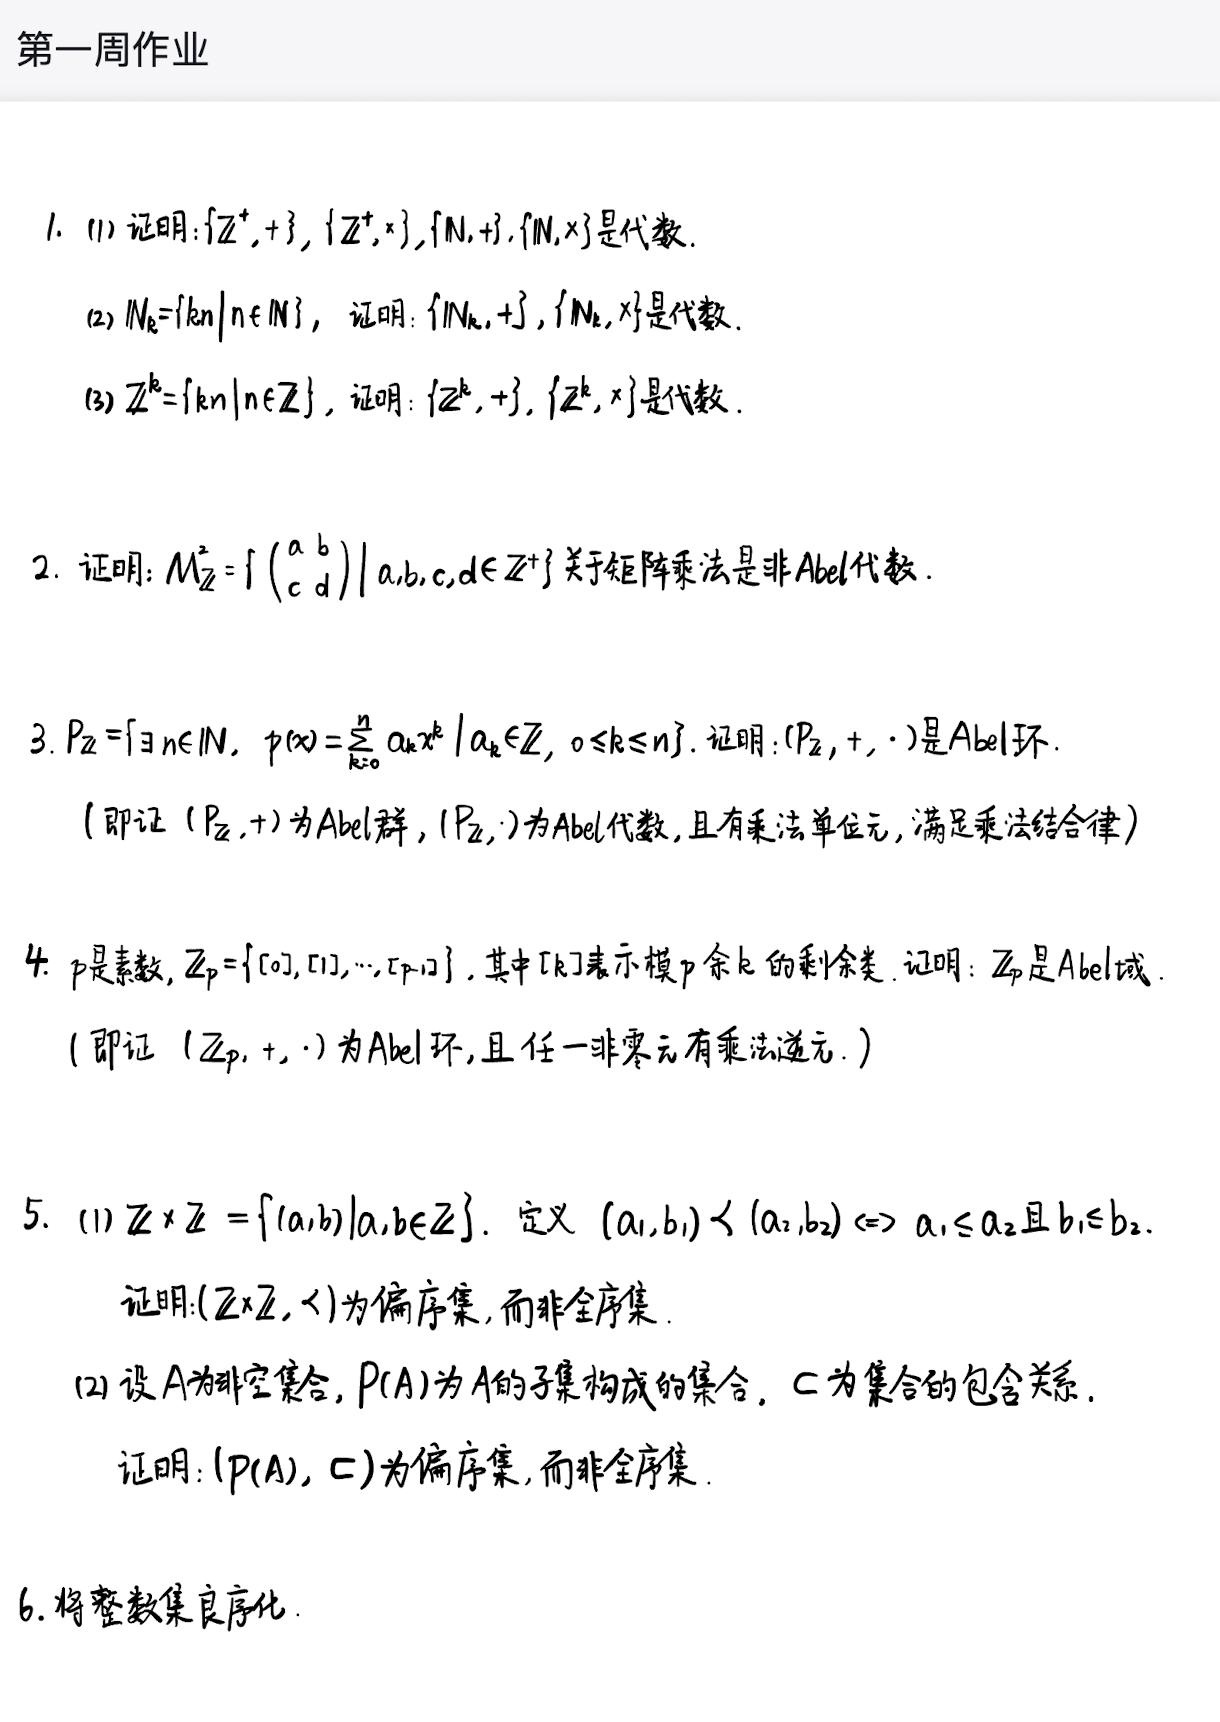
\includegraphics[width=\textwidth]{微信图片_20250301233728.png}
% \caption{}
\label{}
\end{figure}

\begin{exercise}
\begin{enumerate}
		\item 证明:$\{ \mathbb{Z}^{+},+ \},\{ \mathbb{Z}^{+},\times \},\{ \mathbb{N},+ \},\{ \mathbb{N},\times \}$ 是代数。
		\item $\mathbb{N}_{k}=\{ kn|n\in \mathbb{N} \}$ 证明 $\{ \mathbb{N}_{k},+ \},\{ \mathbb{N}_{k},\times \}$ 是代数。
		\item $\mathbb{Z}^{k}=\{ kn|n\in \mathbb{Z} \}$ 证明 $\{ \mathbb{Z}^{k},+ \},\{ \mathbb{Z}^{k},\times \}$ 是代数。
	\end{enumerate}
\end{exercise}
\begin{definition}[代数]
代数是一个非空集合 $A$ 和一个二元运算 $\circ: A \times A \to A$,满足:
封闭性:$\forall a, b \in A$,$a \circ b \in A$
我们通常将代数记为 $(A, \circ)$。
\end{definition}
\begin{enumerate}
	\item 简单验证:
	\begin{enumerate}
		\item $a, b\in \mathbb{Z}^{+}\Rightarrow a+b\in \mathbb{Z}^{+}$
		\item $a, b\in \mathbb{Z}^{+}\Rightarrow a\times b\in \mathbb{Z}^{+}$
		\item $a, b\in \mathbb{N}\Rightarrow a+b\in \mathbb{N}$
		\item $a, b\in \mathbb{N}\Rightarrow a\times\in \mathbb{N}$
	\end{enumerate}
	\item 简单验证:
	\begin{enumerate}
		\item $kn_{1}, kn_{2}\in \mathbb{N}_{k}\Rightarrow kn_{1}+kn_{2}=k (n_{1}+n_{2})\in \mathbb{N}_{k}$
		\item $kn_{1}, kn_{2}\in \mathbb{N}_{k}\Rightarrow kn_{1}\times kn_{2}=k (n_{1}kn_{2})\in \mathbb{N}_{k}$
	\end{enumerate}
	\item 简单验证
	\begin{enumerate}
		\item $kn_{1}, kn_{2}\in \mathbb{Z}_{k}\Rightarrow kn_{1}+kn_{2}=k (n_{1}+n_{2})\in \mathbb{Z}_{k}$
		\item $kn_{1}, kn_{2}\in \mathbb{Z}_{k}\Rightarrow kn_{1}\times kn_{2}=k (n_{1}kn_{2})\in \mathbb{Z}_{k}$
	\end{enumerate}
\end{enumerate}

\begin{exercise}
证明 $M^{2}_{\mathbb{Z}}=\{ \left.\begin{pmatrix}a&b\\c&d\end{pmatrix}\right|a,b,c,d\in \mathbb{Z}^{+} \}$ 关于矩阵乘法是非 Abel 代数
\end{exercise}
首先,我们需要明确非 Abel 代数的定义:

\begin{definition}[非 Abel 代数]
一个代数 $(A, \circ)$ 称为非 Abel 代数(或非交换代数),如果存在 $a, b \in A$,使得 $a \circ b \neq b \circ a$。
\end{definition}
现在证明 $M^{2}_{\mathbb{Z}}$ 关于矩阵乘法是非 Abel 代数:
首先验证 $M^{2}_{\mathbb{Z}}$ 关于矩阵乘法是一个代数:
对于任意 $A, B \in M^{2}_{\mathbb{Z}}$
\[
A=\begin{pmatrix}
a_{1} & b_{1} \\
c_{1} & d_{1} 
\end{pmatrix},B=\begin{pmatrix}
a_{2} & b_{2}  \\
c_{2} & d_{2} 
\end{pmatrix}
\]
我们有矩阵乘法下
\[
AB=\begin{pmatrix}
a_{1}a_{2}+b_{1}c_{2} & a_{1}b_{2}+b_{1}d_{2} \\
c_{1}a_{2}+d_{1}b_{2} & c_{1}b_{2}+d_{1}d_{2}
\end{pmatrix}
\]
其中每个元素都 $\in \mathbb{Z}^{+}$,于是 $AB\in M^{2}_{\mathbb{Z}}$,故 $M^{2}_{\mathbb{Z}}$ 关于矩阵乘法是一个代数。
接下来验证 $M^{2}_{\mathbb{Z}}$ 关于矩阵乘法是非 Abel 代数:
取
\[
A=\begin{pmatrix}
1 & 0 \\
0 & 0
\end{pmatrix},B=\begin{pmatrix}
0 & 1  \\
0  & 1
\end{pmatrix}
\]
于是
\[
AB=\begin{pmatrix}
0 & 1 \\
0 & 0
\end{pmatrix}\neq BA=\begin{pmatrix}
0 & 0  \\
0 & 0
\end{pmatrix}
\]
于是 $M^{2}_{\mathbb{Z}}$ 关于矩阵乘法是非 Abel 代数。

\begin{exercise}
$P_{\mathbb{Z}}=\left\{  \exists n\in \mathbb{N},p(x)=\sum_{k=0}^{n}a_{k}x^{k}|a_{k}\in \mathbb{Z},0\leq k\leq n  \right\}$ 证明 $(P_{\mathbb{Z}},+,\cdot)$ 是 Abel 环
\end{exercise}
即证 $(P_{\mathbb{Z}},+)$ 为 Abel 群,$(P_{\mathbb{Z}},\cdot)$ 为 Abel 代数,且有乘法单位元,满足乘法结合律

\begin{definition}[Abel 环]
Abel 环是指满足以下条件的代数结构 $(R,+,\cdot)$:
	\begin{enumerate}
		\item $(R,+)$ 是 Abel 群
		\item $(R,\cdot)$ 是半群(满足结合律)且有单位元
		\item 乘法对加法满足分配律
		\item 乘法满足交换律(即 $a \cdot b = b \cdot a$,$\forall a,b \in R$)
	\end{enumerate}
\end{definition}
首先验证 $(P_{\mathbb{Z}},+)$ 是 Abel 群:

\begin{enumerate}
	\item 封闭性:对于任意 $p(x), q(x) \in P_{\mathbb{Z}}$,设 $p(x) = \sum_{k=0}^{n}a_{k}x^{k}$,$q(x) = \sum_{k=0}^{m}b_{k}x^{k}$,则 $p(x) + q(x) = \sum_{k=0}^{\max(m,n)}(a_k + b_k)x^k$,其中若 $k > n$ 则 $a_k = 0$,若 $k > m$ 则 $b_k = 0$。由于整数对加法封闭,所以 $a_k + b_k \in \mathbb{Z}$,因此 $p(x) + q(x) \in P_{\mathbb{Z}}$。
	\item 结合律:对于任意 $p(x), q(x), r(x) \in P_{\mathbb{Z}}$,有 $(p(x) + q(x)) + r(x) = p(x) + (q(x) + r(x))$,这是因为多项式系数的加法满足结合律。
	\item 单位元:零多项式 $0 = 0x^0$ 是加法单位元,对任意 $p(x) \in P_{\mathbb{Z}}$,有 $p(x) + 0 = 0 + p(x) = p(x)$。
	\item 逆元:对于任意 $p(x) = \sum_{k=0}^{n}a_{k}x^{k} \in P_{\mathbb{Z}}$,其加法逆元为 $-p(x) = \sum_{k=0}^{n}(-a_{k})x^{k} \in P_{\mathbb{Z}}$,满足 $p(x) + (-p(x)) = 0$。
	\item 交换律:对于任意 $p(x), q(x) \in P_{\mathbb{Z}}$,有 $p(x) + q(x) = q(x) + p(x)$,这是因为多项式系数的加法满足交换律。
\end{enumerate}

接下来验证 $(P_{\mathbb{Z}},\cdot)$ 是 Abel 代数:

\begin{enumerate}
	\item 封闭性:对于任意 $p(x) = \sum_{i=0}^{n}a_{i}x^{i}$,$q(x) = \sum_{j=0}^{m}b_{j}x^{j} \in P_{\mathbb{Z}}$,它们的乘积为 $p(x) \cdot q(x) = \sum_{k=0}^{n+m}c_k x^k$,其中 $c_k = \sum_{i+j=k}a_i b_j$。由于整数对乘法和加法都封闭,所以 $c_k \in \mathbb{Z}$,因此 $p(x) \cdot q(x) \in P_{\mathbb{Z}}$。
	\item 结合律:对于任意 $p(x), q(x), r(x) \in P_{\mathbb{Z}}$,有 $(p(x) \cdot q(x)) \cdot r(x) = p(x) \cdot (q(x) \cdot r(x))$,这是多项式乘法的基本性质。
	\item 单位元:多项式 $1 = 1x^0$ 是乘法单位元,对任意 $p(x) \in P_{\mathbb{Z}}$,有 $p(x) \cdot 1 = 1 \cdot p(x) = p(x)$。
	\item 交换律:对于任意 $p(x), q(x) \in P_{\mathbb{Z}}$,有 $p(x) \cdot q(x) = q(x) \cdot p(x)$,这是因为多项式乘法满足交换律。
\end{enumerate}

最后验证乘法对加法的分配律:
对于任意 $p(x), q(x), r(x) \in P_{\mathbb{Z}}$,有:
$p(x) \cdot (q(x) + r(x)) = p(x) \cdot q(x) + p(x) \cdot r(x)$
$(p(x) + q(x)) \cdot r(x) = p(x) \cdot r(x) + q(x) \cdot r(x)$
综上所述,$(P_{\mathbb{Z}},+,\cdot)$ 是 Abel 环。

\begin{exercise}
$p$ 是素数,$\mathbb{Z}_{p}=\{ [0],[1],\dots,[p-1] \}$,其中 $[k]$ 表示模 $p$ 余 $k$ 的剩余类,证明:$\mathbb{Z}_{p}$ 是 Abel 域
\end{exercise}
即证 $(\mathbb{Z}_{p},+,\cdot)$ 为 Abel 环,且任一非零元有乘法逆元
\begin{figure}[H]
\centering
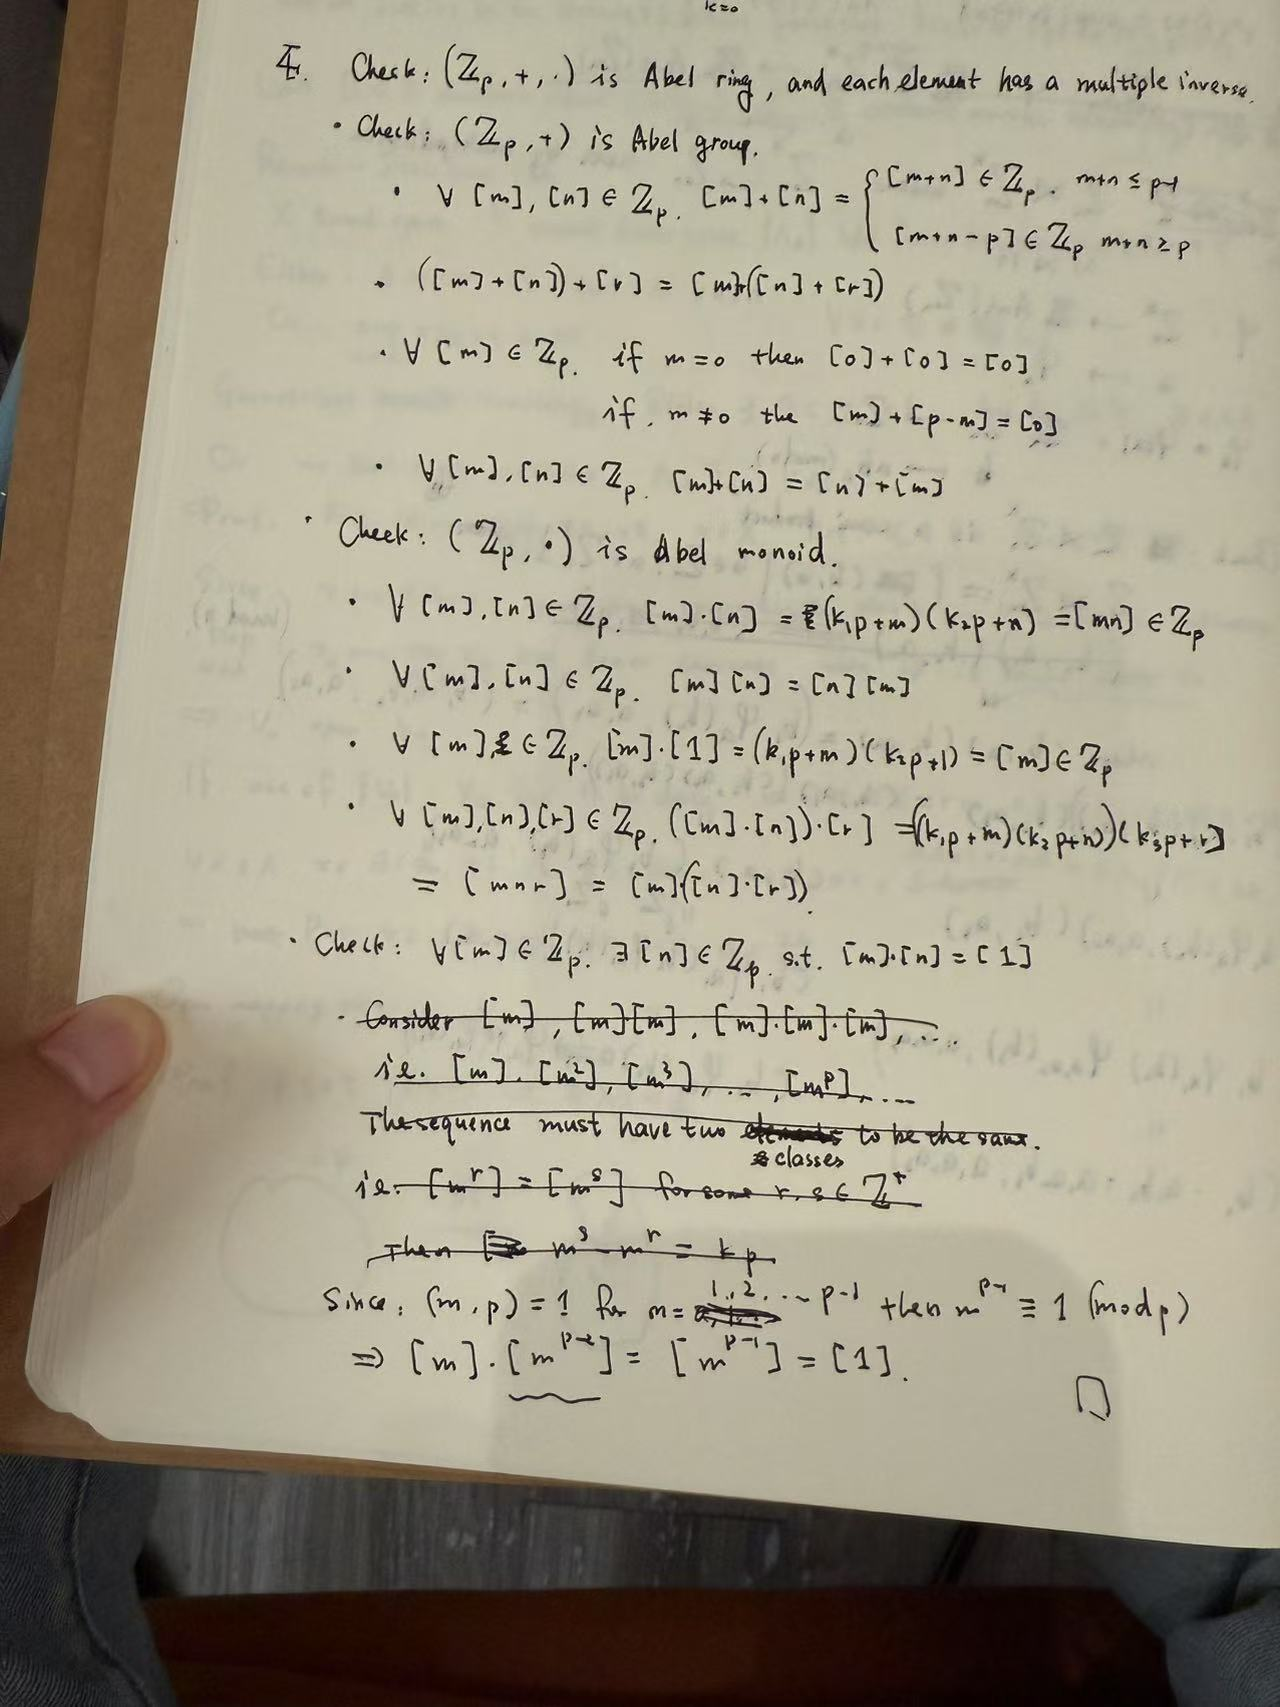
\includegraphics[width=\textwidth]{8f3725a58915a7b2bb9702d910386c1.jpg}
% \caption{}
\label{}
\end{figure}

\begin{exercise}
\begin{enumerate}
		\item $\mathbb{Z}\times \mathbb{Z}=\{ (a,b)|a,b\in \mathbb{Z} \}$ 定义 $(a_{1}, b_{1})\prec (a_{2},b_{2})\iff a_{1}\leq a_{2}\text{ and }b_{1}\leq b_{2}$。证明:$(\mathbb{Z}\times \mathbb{Z},\prec)$ 是偏序集,而非全序集
		\item 设 $A$ 为非空集合,$P(A)$ 为 $A$ 的子集构成的集合,$\subset$ 为集合的包含关系,证明 $P(A,\subset)$ 为偏序集,而非全序集
	\end{enumerate}
\end{exercise}
\begin{figure}[H]
\centering
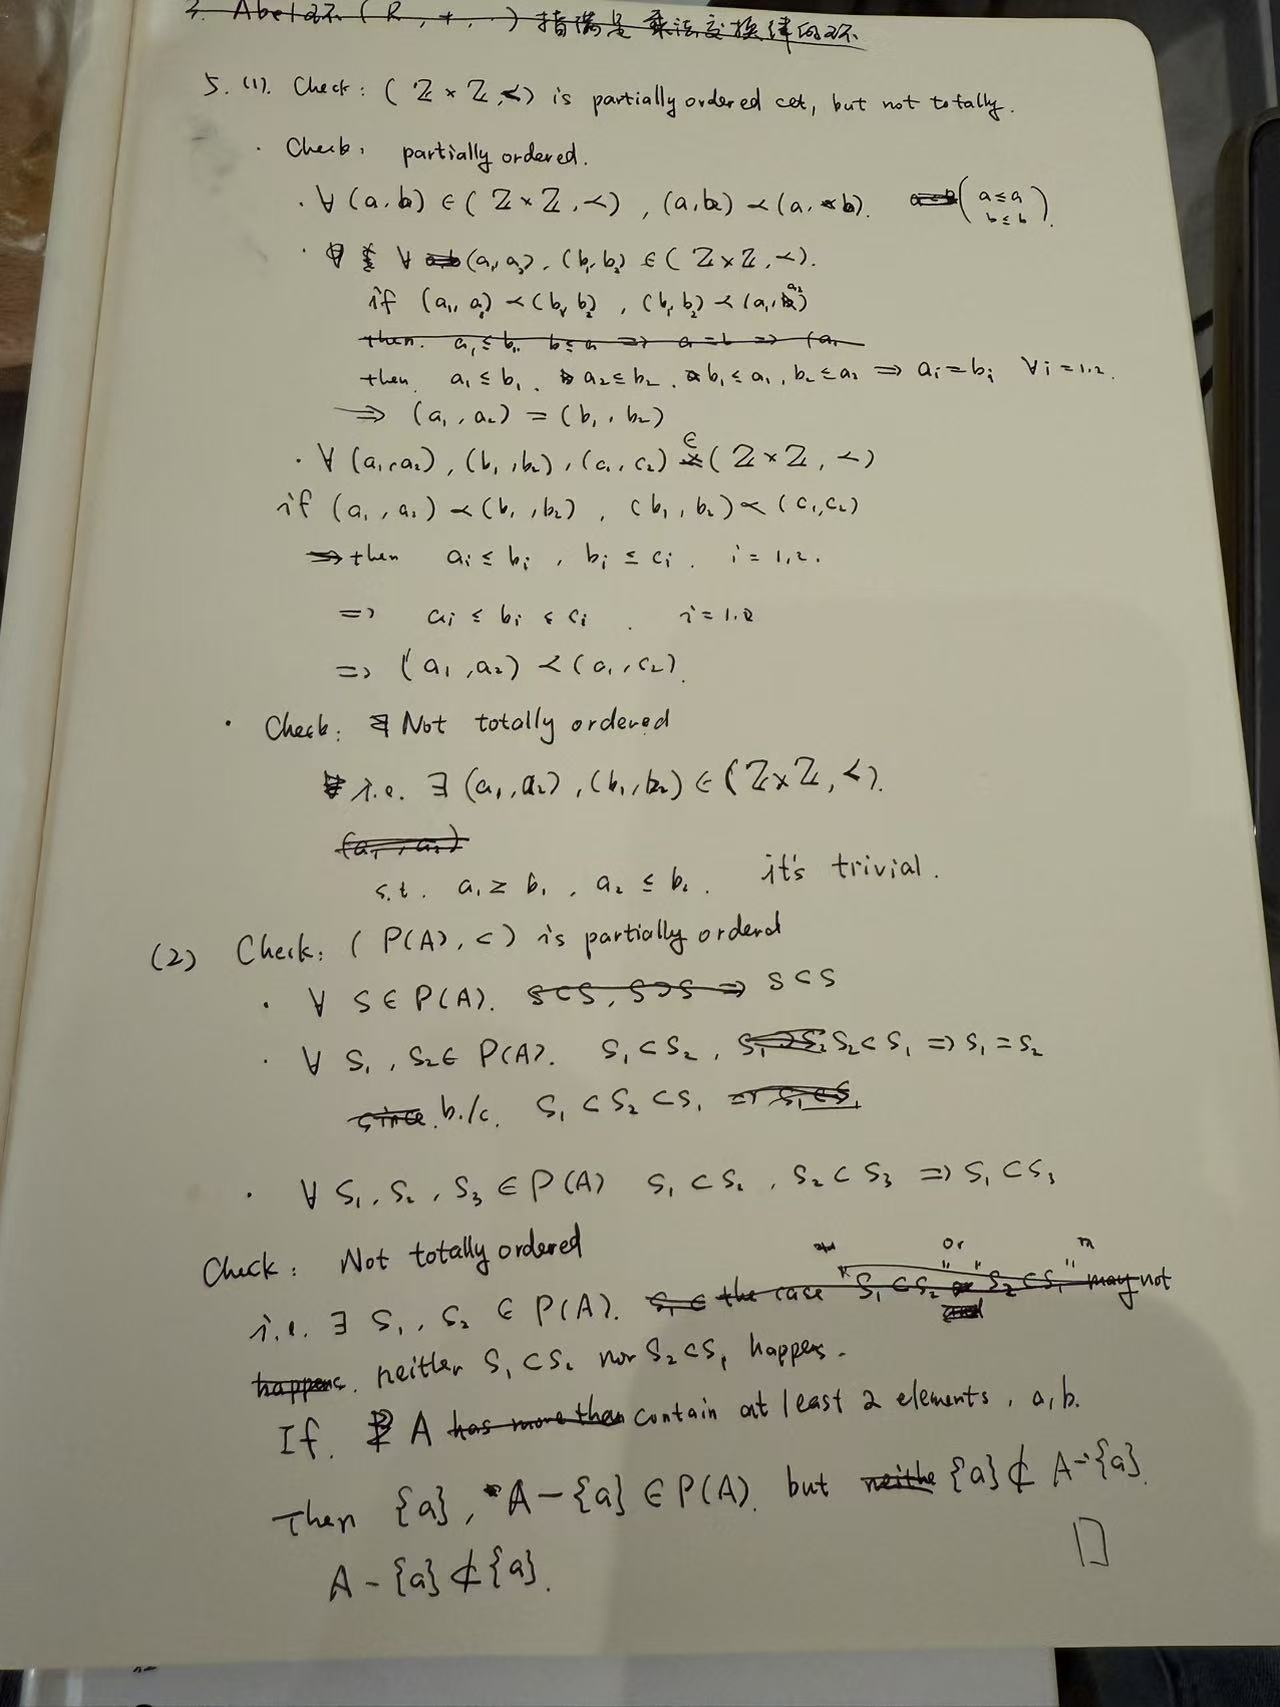
\includegraphics[width=\textwidth]{923f077fa8274b535d8cc207b5812bd.jpg}
% \caption{}
\label{}
\end{figure}

\begin{exercise}
将整数集良序化
\end{exercise}
\begin{figure}[H]
\centering
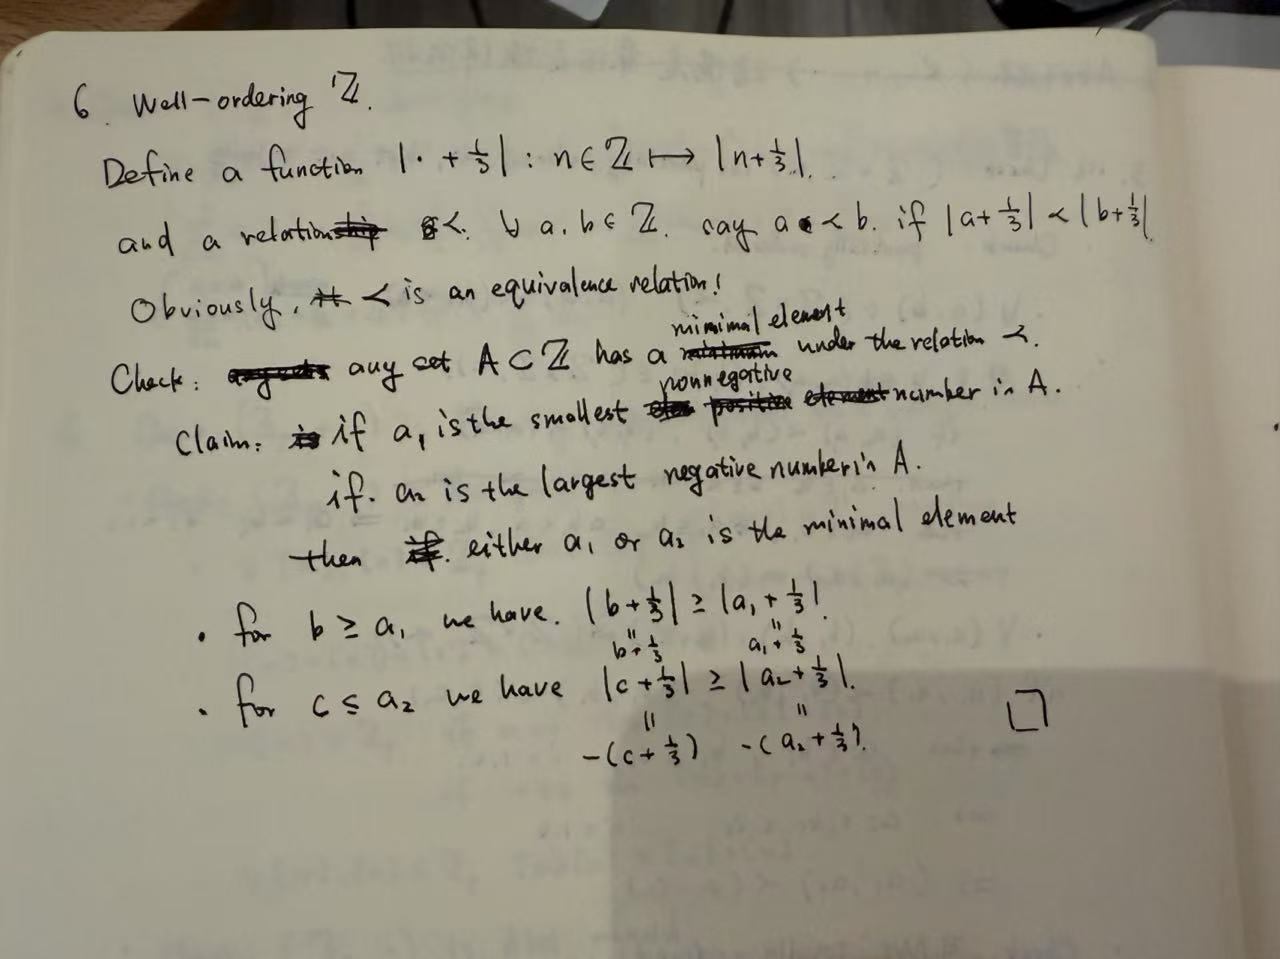
\includegraphics[width=\textwidth]{ad7dab77d435722306c171ed8990669.jpg}
% \caption{}
\label{}
\end{figure}
